\section{Results} \label{Results}

Figure \ref{ResultsPlot} shows the dynamic treatment effects and figure \ref{ResultsPlotSub} shows the same plot for the four subgroups of interest. 

\begin{figure}[!h]
	\centering
	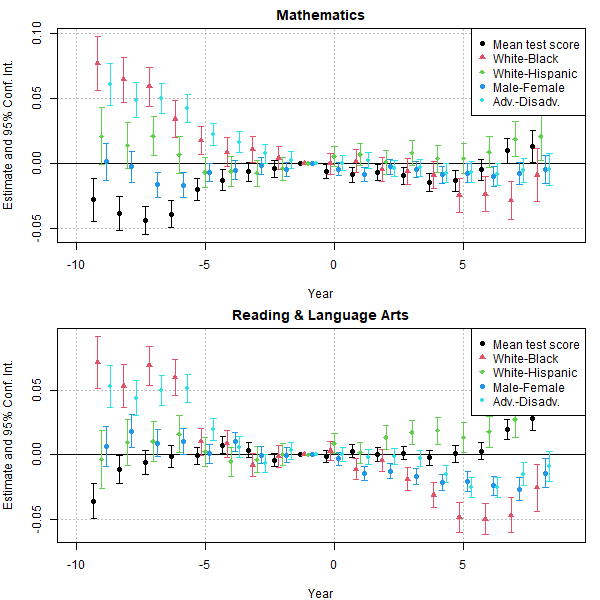
\includegraphics[scale=1]{"../Code & Data/ResultsPlot.png"}
	\caption{Dynamic Treatment effects}
	\label{ResultsPlot}
\end{figure}

\begin{figure}[!h]
	\centering
	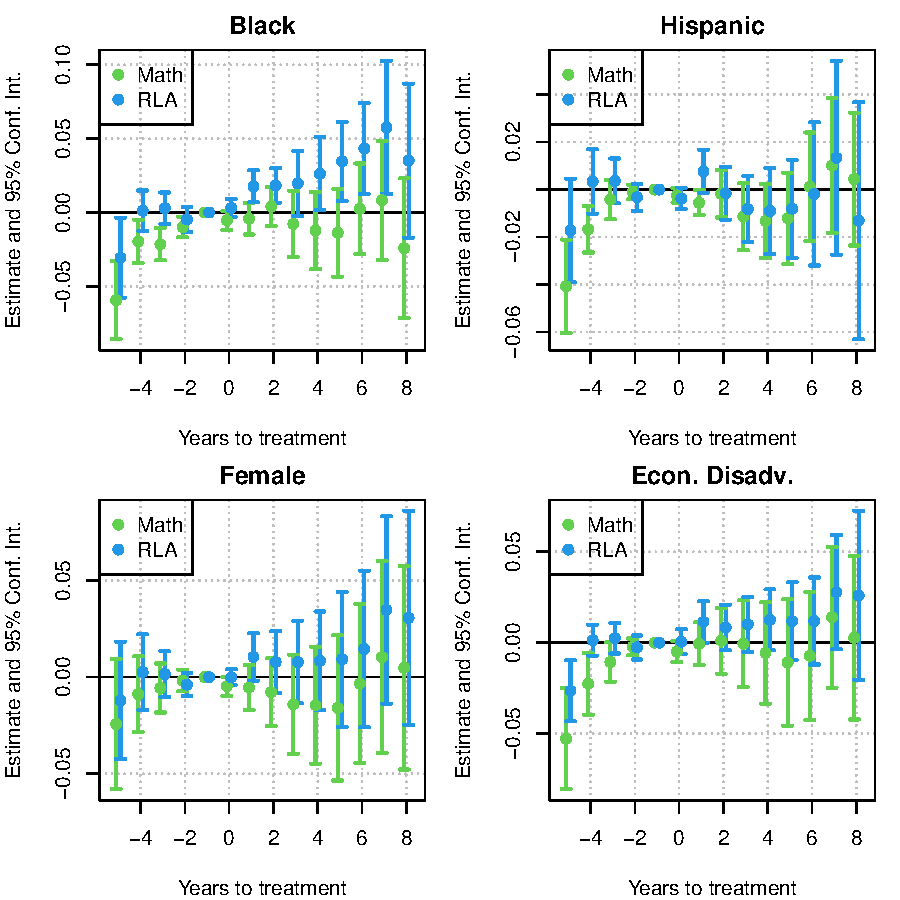
\includegraphics[scale=1]{"../Code & Data/ResultsPlotSub.png"}
	\caption{Dynamic Treatment effects for various subgroups}
	\label{ResultsPlotSub}
\end{figure}


Figures \ref{ResultsPlotStorm} and \ref{ResultsPlotSubStorm} show the same graphs based on the storm treatment.


\begin{figure}[!h]
	\centering
	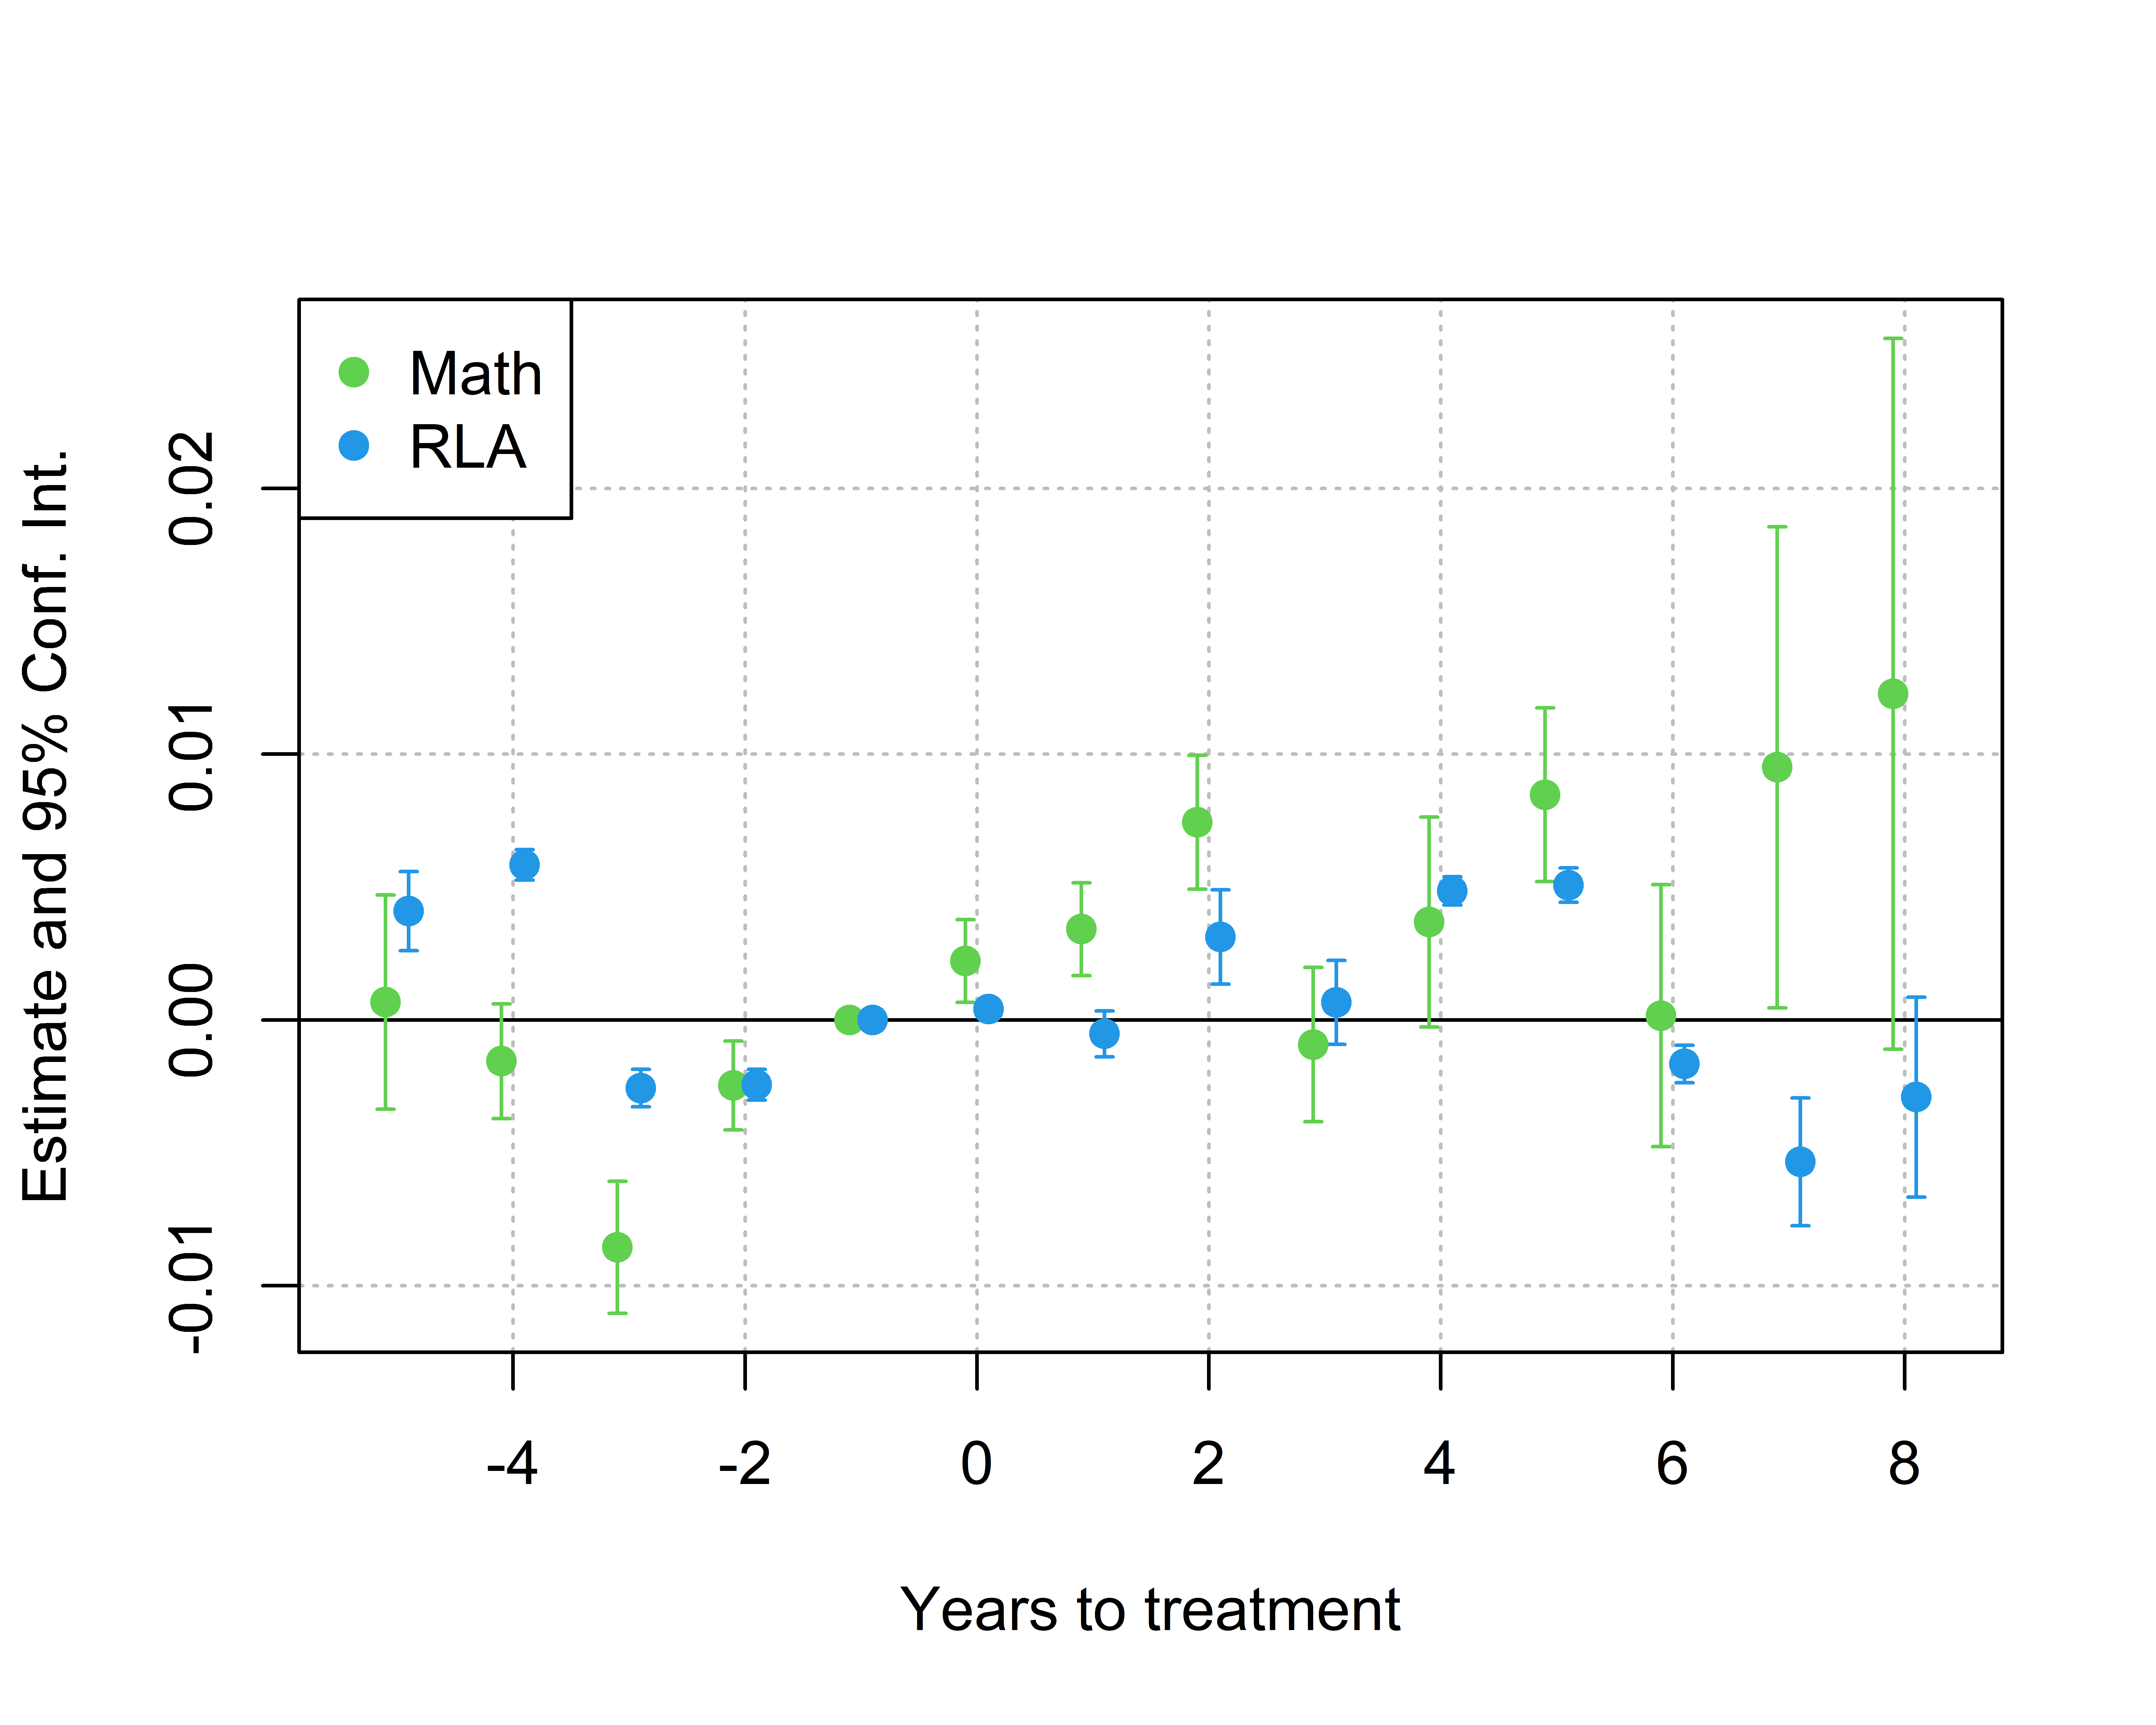
\includegraphics[scale=1]{"../Code & Data/ResultsPlotStorm.png"}
	\caption{Dynamic Treatment effects}
	\label{ResultsPlotStorm}
\end{figure}

\begin{figure}[!h]
	\centering
	\includegraphics[scale=1]{"../Code & Data/ResultsPlotSubStorm.png"}
	\caption{Dynamic Treatment effects for various subgroups}
	\label{ResultsPlotSubStorm}
\end{figure}








